\documentclass[journal,twoside,web]{ieeecolor}

\usepackage{generic}
\usepackage{cite}
\usepackage{amsmath,amssymb,amsfonts}
\usepackage{algorithmic}
\usepackage{graphicx}
\usepackage{textcomp}
\usepackage{mathtools}
\usepackage{graphicx}
\usepackage{subfigure}
\usepackage{epsfig} % for postscript graphics files
\usepackage{cite}
%\usepackage{amsthm}  % assumes amsmath package installed
%\usepackage{widetext}
\usepackage{lcsys}
\usepackage{gensymb}


\newcommand{\sy}[1]{\textcolor{red}{SY: #1}}
\newcommand{\bl}[1]{\textcolor{blue}{#1}}

%---------

%\documentclass[letterpaper, 10pt, conference]{ieeeconf}  % Comment this line out if you need a4paper

%\documentclass[a4paper, 10pt, conference]{ieeeconf}      % Use this line for a4 paper

%\IEEEoverridecommandlockouts                              % This command is only needed if
                                                          % you want to use the \thanks command

\newtheorem{theorem}{Theorem}[section]
\newtheorem{lemma}[theorem]{Lemma}
\newtheorem{proposition}[theorem]{Proposition}
\newtheorem{corollary}[theorem]{Corollary}
\newtheorem{definition}[theorem]{Definition}
\newtheorem{remark}[theorem]{Remark}
\newtheorem{assumption}[theorem]{Assumption}
\newtheorem{problem}[theorem]{Problem}

\pagestyle{empty} % Removes all the page numbers (except for the title page)

% Algorithms 
% \usepackage{algorithm}
% \usepackage[noend]{algpseudocode}
% \newcommand{\algorithmautorefname}{Algorithm}
% \algrenewcommand{\Require}{\Statex \textbf{Input:}}  
% \algrenewcommand{\Ensure}{\Statex \textbf{Output:}} 

\begin{document}


\def\BibTeX{{\rm B\kern-.05em{\sc i\kern-.025em b}\kern-.08em
    T\kern-.1667em\lower.7ex\hbox{E}\kern-.125emX}}
\markboth{\journalname, VOL. XX, NO. XX, XXXX 2017}
{Author \MakeLowercase{\textit{et al.}}: Preparation of Papers for IEEE Control Systems Letters (August 2022)}


\title{Control Synthesis for Security Hyperproperties Using Control Barrier Functions}


%\author{
%Georgios Mitsos$^{a}$,
%Siyuan Liu$^{a}$
%\thanks{$^{a}$ Department of Electrical Engineering, Eindhoven University of Technology, Eindhoven, the Netherlands; \{\texttt{g.mitsos, s.liu5}\}\texttt{@tue.nl}
%}  
%}

\maketitle
\thispagestyle{empty}
 

%%%%%%%%%%%%%%%%%%%%%%%%%%%%%%%%%%%%%%%%%%%%%%%%%%%%%%%%%%%%%%%%%%%%%%%%%%%%%%%%
\begin{abstract}
    Many security and privacy requirements in cyber-physical systems are inherently relational, involving comparisons across multiple system executions rather than properties of single executions. Such requirements, known as hyperproperties, naturally arise in information-flow security and include notions such as opacity, noninterference, and $K$-anonymity. Since such properties cannot, in general, be expressed using standard temporal logics, HyperLTL has emerged as a powerful tool for specifying a broad class of security requirements.
    This paper presents an online control synthesis framework for enforcing hyperproperties in continuous-time control-affine systems using control barrier functions (CBFs). Hyperproperties are encoded in HyperLTL and enforced by constructing CBFs over an augmented state space that captures multiple system executions. The resulting barrier conditions are incorporated as constraints in a quadratic program, enabling real-time controller synthesis with formal guarantees of hyperproperty satisfaction. 
    The proposed framework provides a unified approach for integrating formal information-flow security requirements into continuous-time controller synthesis. We show how representative security notions can be formulated within the proposed framework and synthesize controllers that enforce them online. Finally, case studies demonstrate the effectiveness of the proposed approach.
\end{abstract}

\begin{IEEEkeywords}
    Cyber-physical systems, Hyperproperties, Security, Controller synthesis, Control barrier functions
\end{IEEEkeywords}

\section{Introduction}
\label{sec:introduction}

\IEEEPARstart{A}{utonomous} cyber-physical systems (CPS) increasingly operate in uncertain, dynamic, and potentially adversarial environments where correct behavior must be ensured not only along a single trajectory, but across families of trajectories arising from uncertainty and/or adversarial observation. At the same time, modern robotic systems must accomplish complex tasks while providing formal correctness guarantees. Formal specification and synthesis methods based on temporal logics have therefore become central tools for motion planning and control \cite{fainekos2009, kloetzer2008}, enabling high-level task specification, and fully-automated and correct-by-design controller synthesis \cite{smith2011}.

Standard linear temporal logic (LTL) specifications, however, describe properties of individual executions. Many requirements in robotics and CPS are instead relational, i.e., they compare multiple system executions of the same system \cite{wang2020}. For example, optimality compares trajectories with respect to a given cost criterion, while robustness compares nominal and perturbed executions to ensure that desired system behavior is satisfied despite uncertainty.
Many security and privacy requirements are also inherently relational. Specifically, they ask whether two or more executions can be distinguished by an adversary, and therefore cannot, in general, be expressed as standard single-trace LTL properties.

In this work, we focus on security hyperproperties for CPS. We consider a malicious intruder modeled as an external observer that has only partial access to the system executions through an output function. The intruder does not observe the full state, but attempts to infer hidden information from the observed outputs. This setting naturally captures information-flow security requirements \cite{zhao2024}. Opacity \cite{saboori2007} requires that the intruder cannot determine whether the system has executed a secret behavior, such as visiting a sensitive region.
Noninterference \cite{xiang2021} requires that confidential high-security inputs do not influence low-security outputs observed by the intruder. 
$K$-anonymity \cite{yin2016} requires maintaining $K$ indistinguishable copies of the system such that the intruder cannot infer the execution responsible for a sensitive event. These properties compare what the intruder observes across multiple possible executions and are therefore naturally expressed as hyperproperties \cite{clarkson2010}.

Hyperlogics provide formal languages for specifying such multi-execution requirements. In particular, HyperLTL and HyperCTL extend temporal logics with explicit quantification over traces \cite{clarkson2014}, allowing formulas that relate several system executions through universal and existential quantifiers \cite{finkbeiner2015}. For continuous and real-valued signals, related formalisms such as HyperSTL have also been proposed \cite{nguyen2017}. 

Verification of hyperproperties has advanced substantially via automata-based model checking \cite{clarkson2014}, dedicated tools \cite{finkbeiner2015}, and, more recently, certificate-based approaches \cite{anand2024}. In contrast, control synthesis for hyperproperties has received increasing attention only recently. In both verification and control synthesis, most existing approaches target discrete-event systems (DES) \cite{wang2020, finkbeiner2015}, while recent approaches extend to discrete-time \cite{anand2024, zhao2025} and continuous-time \cite{cui2026} dynamical systems. Similarly, opacity-preserving synthesis is primarily studied for DES \cite{yang2023, yu2022} or discrete-time systems through offline synthesis procedures \cite{zhong2025}. As a result, the online enforcement of security hyperproperties for continuous-time CPS remains largely unexplored.

Continuous-time CPS require real-time control capable of reacting to disturbances and uncertainty during operation. Control barrier functions (CBFs) provide a suitable optimization-based framework for online synthesis of safety-critical controllers by rendering safe sets forward invariant \cite{ames2014, ames2019}. CBFs have also been combined with temporal-logic objectives to enable real-time control for complex tasks \cite{lindemann2019, srinivasan2021}.

This paper develops an online CBF-based control synthesis framework for enforcing security hyperproperties, specified in HyperLTL, for continuous-time control-affine systems. The proposed approach constructs CBF conditions over a self-composed augmented system whose states correspond to the executions quantified in the HyperLTL formula. These conditions are imposed as constraints in a quadratic program (QP), yielding real-time controllers with formal guarantees of hyperproperty satisfaction. 

Compared with existing HyperLTL-based planning methods for robotics, which primarily rely on DES \cite{wang2020, bonakdarpour2022} or discrete-time settings \cite{zhao2025}, our approach addresses online control synthesis directly on continuous-time dynamics. While certificate-based methods for dynamical systems have mainly been developed for verification \cite{anand2024, cui2026}, we use CBFs to synthesize controllers in real time. The proposed framework also goes beyond opacity-preserving synthesis methods \cite{yang2023, yu2022, zhong2025} by providing a unified treatment of several security hyperproperties, including approximate opacity, noninterference, and $K$-anonymity. Finally, the case study demonstrates that these security constraints can be combined with standard LTL task constraints within the same QP.

The remainder of the paper is organized as follows.
Section~\ref{sec:preliminaries} introduces notation and preliminaries. 
Section~\ref{subsec:security} formulates the security hyperproperties considered in this work using HyperLTL and develops the CBF conditions to enforce them. 
Section~\ref{sec:control} presents the QP-based control synthesis framework that guarantees satisfaction of the hyperproperties.
Section~\ref{sec:case_study} illustrates the proposed framework through robot case studies, and Section~\ref{sec:conclusion} concludes the paper.

\section{Preliminaries}
\label{sec:preliminaries}

\textbf{Notation.} Let $\mathbb{R}$ and $\mathbb{N}$ denote the sets of real numbers and positive integers, respectively. Let $\mathbb{R}_{\ge 0}$ denote the set of nonnegative real numbers. For $n, m \in \mathbb{N}$, $\mathbb{R}^n$ denotes the space of $n$-dimensional column vectors, and $\mathbb{R}^{n \times m}$ the space of $n \times m$ real matrices. Vectors are denoted by bold lowercase letters and matrices by bold uppercase letters.The zero vector in $\mathbb{R}^n$ and matrix in $\mathbb{R}^{n \times m}$ are denoted by $\mathbf{0}_n$ and $\mathbf{0}_{n \times m}$, respectively. For $\mathbf{x} = \begin{bmatrix} x_1 & \dots & x_n \end{bmatrix}^\top \in \mathbb{R}^n$, $\|\mathbf{x}\|$ denotes the Euclidean norm, i.e., $\|\mathbf{x}\| = \sqrt{\mathbf{x}^\top \mathbf{x}}$. The notation $\operatorname{diag}(\lambda_1, \lambda_2, \dots)$ denotes a diagonal matrix with entries $\lambda_1, \lambda_2, \dots$. A continuous function $\alpha: \mathbb{R}_{\ge 0} \to \mathbb{R}_{\ge 0}$ is said to be of class-$\mathcal{K}$ if it is strictly increasing and satisfies $\alpha(0) = 0$. The symbol for a continuously differentiable is $\mathbf{C}^1$. Given a $\mathbf{C}^1$ function $V : \mathbb{R}^n \to \mathbb{R}$ and a vector field $\mathbf{f} : \mathbb{R}^n \to \mathbb{R}^n$ , the Lie derivative of $V$ along $\mathbf{f}$ is defined as $L_\mathbf{f} V(\mathbf{x}) = \tfrac{\partial V}{\partial \mathbf{x}} \mathbf{f}(\mathbf{x})$. Similarly, for a matrix field $\mathbf{G} : \mathbb{R}^n \to \mathbb{R}^{n \times m}$, we define
$L_{\mathbf{G}}V(\mathbf{x}) = \frac{\partial V}{\partial \mathbf{x}} \mathbf{G}(\mathbf{x})$.

\subsection{System model} \label{subsec:system}

We consider a nonlinear input-affine control system
\begin{equation} \label{eq:system}
    S: \quad \dot{\mathbf{x}} = \mathbf{f}(\mathbf{x}) + \mathbf{G}(\mathbf{x}) \, \mathbf{u}, \quad \mathbf{x}(0) = \mathbf{x}_0.
\end{equation}
where $\mathbf{x} \in \mathbb{X} \subseteq \mathbb{R}^n$ is the state and $\mathbf{u} \in \mathbb{U} \subseteq \mathbb{R}^m$ is the control input. The initial state $\mathbf{x}_0$ satisfies $\mathbb{X}_0 \subseteq \mathbb{X} \subseteq \mathbb{R}^n$. The functions $\mathbf{f}: \mathbb{R}^n \rightarrow \mathbb{R}^n$ and $\mathbf{G}: \mathbb{R}^n \rightarrow \mathbb{R}^{n \times m}$ are locally Lipschitz continuous.

Given a controller $\boldsymbol{\nu}: \mathbb{R}_{\ge 0} \to \mathbb{U}$ and an initial state $\mathbf{x}_0 \in \mathbb{X}_0$, we denote by
$\mathbf{x}_{\mathbf{x}_0,\boldsymbol{\nu}}: \mathbb{R}_{\ge 0} \to \mathbb{X}$
the corresponding closed-loop trajectory of \eqref{eq:system} under $\boldsymbol{\nu}$, with $\mathbf{x}_{\mathbf{x}_0,\boldsymbol{\nu}}(0)=\mathbf{x}_0$.

We consider a passive malicious intruder that externally observes the system through an output map
$\mathbf{y} = \mathbf{h}(\mathbf{x})$,
where $\mathbf{y} \in \mathbb{Y} \subseteq \mathbb{R}^q$ is the observed output and $\mathbf{h}: \mathbb{X} \to \mathbb{Y}$ is $\mathbf{C}^1$. For $\mathbf{x}_{\mathbf{x}_0,\boldsymbol{\nu}}(t)$, the corresponding output trajectory is 
\begin{equation} \label{eq:output}
    \mathbf{y}_{\mathbf{x}_0, \boldsymbol{\nu}} (t) = \mathbf{h} \big( \mathbf{x}_{\mathbf{x}_0, \boldsymbol{\nu}} (t) \big), \quad \forall t \in \mathbb{R}_{\ge 0}.
\end{equation}

The system model in \eqref{eq:system} and the output trajectory are available to the intruder. Based on this, the intruder attempts to infer secret information about the system, e.g., whether a secret region has been visited, whether confidential actions influence observed outputs, or which execution is responsible for a sensitive event. These requirements compare the observed behavior of multiple possible executions and will be formalized later as security hyperproperties. 

\subsection{Control barrier functions}

Consider a system as in \eqref{eq:system} and a set $\mathcal{C} \subseteq \mathbb{X}$ defined as the superlevel set of a $\mathbf{C}^1$ function $b: \mathbb{R}^n \to \mathbb{R}$, i.e., 
\begin{equation} \label{eq:safe_set}
    \mathcal{C} := \{\mathbf{x} \in \mathbb{X} \mid b(\mathbf{x}) \ge 0 \}.
\end{equation}  
\begin{definition}\label{def:cbf}
    Let $\mathcal{C}$ be defined as in \eqref{eq:safe_set}. The function $b$ is a CBF if there exists a locally Lipschitz class-$\mathcal{K}$ function $\alpha$ such that 
    \begin{equation} \label{eq:cbf}
       \sup_{\mathbf{u} \in \mathbb{U}} \Big[ L_\mathbf{f} b ( \mathbf{x}) + L_\mathbf{G} b ( \mathbf{x}) \, \mathbf{u} \Big] \ge -\alpha(b(\mathbf{x})), \ \forall \mathbf{x} \in \mathbb{X}.
    \end{equation}
\end{definition}

\begin{theorem} \label{thm:forward_invariance}
    \cite{ames2019} Let $\mathcal{C} \subseteq \mathbb{X}$ be defined as the superlevel set of a $\mathbf{C}^1$ function $b: \mathbb{R}^n \rightarrow \mathbb{R}$. If $b$ is a CBF, then any Lipschitz continuous controller $\mathbf{u}(\mathbf{x})$ satisfying $L_\mathbf{f} b ( \mathbf{x}) + L_\mathbf{G} b ( \mathbf{x}) \, \mathbf{u} \!\ge\! -\alpha(b(\mathbf{x}))$ renders $\mathcal{C}$ forward invariant for \eqref{eq:system}, i.e., $\mathbf{x}(0) \in \mathcal{C}$ implies $\mathbf{x}(t) \in \mathcal{C} $ for all $t \in \mathbb{R}_{\ge 0}$.
\end{theorem}

\subsection{Linear temporal logic}

\subsubsection{LTL}

Let $\mathcal{AP}$ be a finite set of atomic propositions. The syntax of LTL is defined recursively as in \cite{baier2008}:
\begin{equation*} \label{eq:ltl}
    \varphi \Coloneqq \pi \mid \lnot \, \varphi \mid \varphi_1 \land \varphi_2 \mid \varphi_1 \, \mathcal{U} \, \varphi_2,
\end{equation*}
where $\pi \in \mathcal{AP}$, and $\varphi$, $\varphi_1$, $\varphi_2$ are LTL formulas, and $\mathcal{U}$ denotes the \emph{until} operator. The Boolean disjunction and \emph{true}, and the temporal operators \emph{eventually} and \emph{always} are defined in the standard way \cite{baier2008}. The $\emph{next}$ operator is omitted since it is not meaningful for continuous-time systems.

A trace is an infinite word $\sigma = \sigma[1] \sigma[2] \dots$, where $\sigma[i] \in 2^\mathcal{AP}$, $\forall i \in \mathbb{N}$. The set of all traces is denoted by $\Sigma^\omega = (2^\mathcal{AP})^\omega$. Satisfaction of an LTL formula $\varphi$ by a trace $\sigma$ is denoted by $\sigma \models \varphi$ and follows the standard LTL semantics \cite{baier2008}.

\subsubsection{HyperLTL}

HyperLTL extends LTL by allowing explicit quantification over multiple traces. Its syntax is given by \cite{clarkson2014}:
\begin{equation*} \label{eq:hyperltl}
    \begin{aligned}
        \psi &\Coloneqq \exists \tau. \psi \mid \forall \tau .  \psi \mid \varphi \\
        \varphi &\Coloneqq \pi_\tau \mid \lnot \, \varphi \mid \varphi_1 \land \varphi_2 \mid \varphi_1 \, \mathcal{U} \, \varphi_2,
    \end{aligned}
\end{equation*}
where $\tau$ is a trace variable and $\pi_\tau$ denotes that proposition $\pi \in \mathcal{AP}$ holds on the trace assigned to $\tau$. 
% The formula $\psi$ denotes a HyperLTL formula, while $\varphi$ denotes its quantifier-free temporal part. 

Let $\mathbb{T}$ be a set of trace variables, and $\mathbb{S} \subseteq \Sigma^\omega$ a set of traces. A trace assignment $V: \mathbb{T} \to \mathbb{S}$ maps trace variables to traces in $\mathbb{S}$. We denote by $V[\tau \mapsto \sigma]$ the assignment that maps $\tau \in \mathbb{T}$ to $\sigma \in \mathbb{S}$ and agrees with $V$ on all other trace variables. For $j \in \mathbb{N}$, $V[j, \infty]$ is the suffix of the trace $V(\tau)$ starting at position $j$, i.e., $V(\tau)[j, \infty]$ for all $\tau \in \mathbb{T}$. 

Given a set of traces $\mathbb{S}$ and a trace assignment $V$, satisfaction of a HyperLTL formula $\psi$ is defined as in \cite{clarkson2014}:
\begin{equation*}
    \begin{aligned}
        &V \models_\mathbb{S} \pi_\tau &\Leftrightarrow& \ \pi \in V(\tau)[0] \\
        &V \models_\mathbb{S} \neg \varphi &\Leftrightarrow& \ V \not\models_\mathbb{S} \varphi \\
        &V \models_\mathbb{S} \varphi_1 \land \varphi_2 &\Leftrightarrow&  \ V \models_\mathbb{S} \varphi_1 \text{ and }  V \models_\mathbb{S} \varphi_2 \\
        &V \models_\mathbb{S} \varphi_1 \mathcal{U} \varphi_2 &\Leftrightarrow& \ \exists i \in \mathbb{N} \text{ such that } V[i, \infty] \models_\mathbb{S} \varphi_2 \\
        & & & \text{ and } \  V[j, \infty] \models_\mathbb{S} \varphi_1, \ \forall j < i \\
        &V \models_\mathbb{S} \exists \tau. \psi &\Leftrightarrow& \ \exists \sigma \in \mathbb{S} \text{ such that } V[\tau \mapsto \sigma] \models_\mathbb{S} \psi \\
        &V \models_\mathbb{S} \forall \tau. \psi &\Leftrightarrow& \ V[\tau \mapsto \sigma] \models_\mathbb{S} \psi, \ \forall \sigma \in \mathbb{S}.
    \end{aligned}
\end{equation*}
A set of traces $\mathbb{S}$ satisfies $\psi$, denoted $\mathbb{S} \models \psi$, if $V_\emptyset \models_{\mathbb{S}} \psi$, where $V_\emptyset$ is the empty trace assignment.

Each atomic proposition $\pi \in \mathcal{AP}$ is associated with a $\mathbf{C}^1$ predicate function $b_\pi: \mathbb{R}^n \to \mathbb{R}$, and $\pi$ is satisfied at a state $\mathbf{x}$ if and only if $b_\pi(\mathbf{x}) \ge 0$. Although LTL and HyperLTL are defined over discrete traces, the trace assignment $V$ can be extended to continuous-time trajectories (see, e.g., Def.~4 in \cite{kloetzer2008}). A trajectory $\mathbf{x}_{\mathbf{x}_0, \boldsymbol{\nu}}(t)$ induces a trace $\sigma = \sigma[1] \sigma[2] \dots \in \Sigma^\omega$, that represents the propositions satisfied along the trajectory. 
Given a collection of closed-loop trajectories of the system $S$ in \eqref{eq:system}, let $\mathbb{S}_S \subseteq \Sigma^\omega$ denote the corresponding set of induced traces. We write $S \models \psi$ if $\mathbb{S}_S \models \psi$.

HyperLTL formulas can be written in prenex form as
\begin{equation*} 
    \psi = \mu_1 \tau_1 \, \mu_2 \tau_2 \dots \mu_p \tau_p. \, \varphi(\tau_1, \tau_2, \dots, \tau_p), 
\end{equation*}
where $\mu_i \in \{\forall, \exists\}$ for all $i \in \{1, \dots, p\}$ and $\varphi$ is a quantifier-free formula. In this work, we focus on security hyperproperties of the form
\begin{equation} \label{eq:security_hyperltl}
    \psi = \forall \tau_1 \, \exists \tau_2 \dots \exists \tau_p. \, \varphi(\tau_1, \tau_2, \dots, \tau_p), 
\end{equation}
where $\varphi = \square \, \phi$ and $\phi$ contains conjunctions, disjunctions and negations of propositions. Moreover, $\tau_1$ represents the real execution, while $\tau_2,\dots,\tau_p$ are dynamically feasible executions that provide plausible alternatives of the observed behavior and conceal secret behaviors from the intruder. Thus, for every feasible $\tau_1$, the specification requires the existence of $p-1$ alternative executions, possibly depending on $\tau_1$, such that the relational property encoded by $\varphi$ is satisfied. Properties whose objective is to infer task-relevant information \cite{cui2026}, such as detectability, observability, and diagnosability, are outside the scope of this work and are left for future research.

\subsection{Problem formulation}

We first form the $p$-fold self-composition of \eqref{eq:system} by introducing the augmented state and input spaces $\bar{\mathbb{X}} \coloneqq \mathbb{X} \times \dots \times \mathbb{X} $ and $\bar{\mathbb{U}} \coloneqq \mathbb{U} \times \dots \times \mathbb{U}$, with augmented state and input
\begin{equation*}
    \bar{\mathbf{x}} = (\mathbf{x}_1, \dots, \mathbf{x}_p) = \begin{bmatrix} \mathbf{x}_1^\top & \dots & \mathbf{x}_p^\top \end{bmatrix}^\top \in \bar{\mathbb{X}}, \text{ and}
\end{equation*}
\vspace{-4mm}
\begin{equation*}
    \bar{\mathbf{u}} = (\mathbf{u}_1, \dots, \mathbf{u}_p) = \begin{bmatrix} \mathbf{u}_1^\top & \dots & \mathbf{u}_p^\top \end{bmatrix}^\top \in \bar{\mathbb{U}}.
\end{equation*}
The augmented dynamics are $\dot{\bar{\mathbf{x}}} = \bar{\mathbf{f}}(\bar{\mathbf{x}}) + \bar{\mathbf{G}}(\bar{\mathbf{x}}) \, \bar{\mathbf{u}}$, where 
\begin{equation} \label{eq:augmented_system}
    \begin{aligned}
        \bar{\mathbf{f}}(\bar{\mathbf{x}}) &= \begin{bmatrix}
        \mathbf{f}(\mathbf{x}_1)^\top & \dots & \mathbf{f}(\mathbf{x}_p)^\top \end{bmatrix}^\top, \text{ and} \\ 
        \bar{\mathbf{G}}(\bar{\mathbf{x}}) &= \operatorname{diag} \big( \mathbf{G}(\mathbf{x}_1), \dots, \mathbf{G}(\mathbf{x}_p) \big).
    \end{aligned}
\end{equation}
Each trace variable $\tau_i$ corresponds to the trajectory of the $i$-th copy of the system, i.e., $\mathbf{x}_{\mathbf{x}_{0, i}, \boldsymbol{\nu}_i}(t)$ and induces a trace $\sigma_i$.

\begin{problem}
\label{pr:security_hyperproperty}
    Consider $p$ copies of the system $S$ in \eqref{eq:system} with initial conditions $\mathbf{x}_{0, i} \in \mathbb{X}_0$, $i = 1, \dots, p$ and a HyperLTL formula $\psi$ of the form \eqref{eq:security_hyperltl}. Synthesize controllers $\boldsymbol{\nu}_i: \mathbb{R}_{\ge 0} \to \mathbb{U}$, $i=1, \dots, p$ such that $S \models \psi$.
\end{problem}

\section{Security properties in HyperLTL}
\label{sec:security}

The security requirements considered in this paper are observational \cite{cui2026}: they constrain what a passive intruder can infer about the system from the observed output trajectory. We first introduce approximate indistinguishability, which is the basic relation used to compare executions from the intruder's viewpoint, and show how it can be encoded as a CBF constraint on the augmented system \eqref{eq:augmented_system}. We then define security hyperproperties that build on this relation, namely approximate opacity, noninterference, and $K$-anonymity, and express them as HyperLTL formulas.

\subsection{Indistinguishability} \label{subsec:indistinguishability}

Indistinguishability requires two trajectories to generate sufficiently similar observations so that the intruder cannot distinguish between them. We formalize this notion as follows.

\begin{definition} \label{def:approx_indistinguishability}
Consider two trajectories $\mathbf{x}_{\mathbf{x}_{0,i}, \boldsymbol{\nu}_i}$ and
$\mathbf{x}_{\mathbf{x}_{0,j}, \boldsymbol{\nu}_j}$ of \eqref{eq:system} and their outputs given in \eqref{eq:output}. For $\delta > 0$, the two trajectories are said to be $\delta$-\emph{approximately indistinguishable} if
    \begin{equation} \label{eq:indistinguishability}
        \left\| \mathbf{h} \big( \mathbf{x}_{\mathbf{x}_{0,i}, \boldsymbol{\nu}_i}(t)\big) - \mathbf{h} \big( \mathbf{x}_{\mathbf{x}_{0,j}, \boldsymbol{\nu}_j}(t) \big) \right\| \le \delta, \quad \forall t\in\mathbb{R}_{\ge 0}.
    \end{equation}
\end{definition}

The parameter $\delta$ models the measurement precision of the intruder. For trace variables $\tau_i$ and $\tau_j$, we use $\mathsf{Ind}_{\delta}^{ij}$ to denote the predicate induced by $\| \mathbf{h} \big( \mathbf{x}_{\mathbf{x}_{0,i}, \boldsymbol{\nu}_i}(t) \big) - \mathbf{h} \big( \mathbf{x}_{\mathbf{x}_{0,j}, \boldsymbol{\nu}_j}(t) \big) \| \le \delta$ for some $t \in \mathbb{R}_{\ge 0}$. Here, $\mathbf{h}(\mathbf{x}_{\mathbf{x}_{0,i}, \boldsymbol{\nu}_i})$ is the output associated with the trajectory $\mathbf{x}_{\mathbf{x}_{0,i}, \boldsymbol{\nu}_i}$ assigned to trace variable $\tau_i$.

We now want to construct CBF-based constraints expressed on the augmented system $\bar{\mathbb{X}} = \mathbb{X} \times \mathbb{X}$ to enforce indistinguishability. Condition \eqref{eq:indistinguishability} must be expressed with a $\mathbf{C}^1$ function over $\bar{\mathbb{X}}$ and then forward invariance of the corresponding superlevel set must be enforced. The Euclidean norm in \eqref{eq:indistinguishability} is nondifferentiable when $\mathbf{h}(\mathbf{x}_i) = \mathbf{h}(\mathbf{x}_j)$. Using the squared norm leads to a $\mathbf{C}^1$ predicate function
\begin{equation} \label{eq:ind_cbf}
    b_{ij}^{\mathrm{ind}}(\bar{\mathbf{x}}) = \delta^2 - \| \mathbf{h}(\mathbf{x}_i) - \mathbf{h}(\mathbf{x}_j)\|^2 .
\end{equation}
Then, $b_{ij}^{\mathrm{ind}}(\bar{\mathbf{x}})\ge 0$ if and only if $\mathsf{Ind}_{\delta}^{ij}$ is satisfied. 
\begin{proposition} \label{prop:forward_invariance}
    Consider a continuously differentiable function $b: \bar{\mathbb{X}} \to \mathbb{R}$. The CBF condition over the augmented system \eqref{eq:augmented_system} is
    \begin{equation}
    \label{eq:augmented_cbf_condition}
        L_{\bar{\mathbf{f}}} b(\bar{\mathbf{x}}) + L_{\bar{\mathbf{G}}} b(\bar{\mathbf{x}}) \, \bar{\mathbf{u}} \ge -\alpha \big( b(\bar{\mathbf{x}}) \big),
    \end{equation}
    where $\alpha$ is a class-$\mathcal{K}$ function. If \eqref{eq:augmented_cbf_condition} is satisfied for all time and the initial augmented state belongs to the corresponding superlevel set $\mathcal{C} = \big\{ \bar{\mathbf{x}} \in \bar{\mathbb{X}} \mid b(\bar{\mathbf{x}})\ge 0 \big\}$, then $\mathcal{C}$ is forward invariant.
\end{proposition}

Using Proposition~\ref{prop:forward_invariance}, forward invariance of the set $\mathcal{C}_{ij}^{\mathrm{ind}} = \big\{ \bar{\mathbf{x}} \in \bar{\mathbb{X}} \mid b_{ij}^{\mathrm{ind}}(\bar{\mathbf{x}})\ge 0 \big\}$ is enforced by
\begin{equation}
\label{eq:ind_cbf_constraint}
    L_{\bar{\mathbf{f}}} b_{ij}^{\mathrm{ind}}(\bar{\mathbf{x}}) + L_{\bar{\mathbf{G}}} b_{ij}^{\mathrm{ind}}(\bar{\mathbf{x}}) \, \bar{\mathbf{u}} \ge -\alpha_{ij} \! \left( b_{ij}^{\mathrm{ind}} (\bar{\mathbf{x}}) \right).
\end{equation}

\subsection{Security hyperproperties} \label{subsec:security}

We next formulate the security hyperproperties in HyperLTL and derive the corresponding CBF constraints. The construction encodes each predicate in the HyperLTL formulas as a $\mathbf{C}^1$ function over the augmented state space, and enforces forward invariance of the associated superlevel set.

\subsubsection{Approximate opacity}

Consider the system in \eqref{eq:system}. The objective is to prevent the intruder described in \ref{subsec:system}, to infer whether the system trajectory has visited a prescribed secret set
\begin{equation} \label{eq:secret_set}
    \mathbb{X}_s = \{ \mathbf{x} \in \mathbb{X} \mid b_s(\mathbf{x}) < 0 \},
\end{equation}
where $b_s:\mathbb{R}^n \to \mathbb{R}$ is $\mathbf{C}^1$. We denote by $s(\tau)$ the proposition that the trajectory associated with $\tau$ lies in $\mathbb{X}_s$.

\begin{definition} \label{def:opacity}
    Consider the system in \eqref{eq:system}, an initial condition $\mathbf{x}_{0,1} \in \mathbb{X}_0$, and $\delta>0$. The system is \emph{$\delta$-approximate infinite-horizon opaque} if there exist an initial condition $\mathbf{x}_{0,2} \in \mathbb{X}_0$ and controllers $\boldsymbol{\nu}_1$, $\boldsymbol{\nu}_2: \mathbb{R}_{\ge 0} \rightarrow \mathbb{U}$ such that $\mathbf{x}_{\mathbf{x}_{0,1}, \boldsymbol{\nu}_1}(t)$ and $\mathbf{x}_{\mathbf{x}_{0,2}, \boldsymbol{\nu}_2}(t)$ are $\delta$-approximately indistinguishable and
    \begin{equation*}
        \mathbf{x}_{\mathbf{x}_{0,1}, \boldsymbol{\nu}_1}(t) \in \mathbb{X}_s \Rightarrow \mathbf{x}_{\mathbf{x}_{0,2}, \boldsymbol{\nu}_2}(t) \notin \mathbb{X}_s, \quad \forall t \in \mathbb{R}_{\ge 0}.
    \end{equation*}
\end{definition}
Thus, whenever the real trajectory $\mathbf{x}_{\mathbf{x}_{0,1}, \boldsymbol{\nu}_1}$ visits the secret set, there exists an alternative trajectory $\mathbf{x}_{\mathbf{x}_{0,2}, \boldsymbol{\nu}_2}$ that is indistinguishable to the intruder and non-secret at the same time. Hence, the intruder cannot infer whether the secret visit has occurred. This property is the continuous-time analogue of $\delta$-approximate infinite-step opacity \cite{yin2021}. The corresponding HyperLTL formula is
\begin{equation}
\label{eq:hyperltl_opacity}
    \psi_{\mathrm{op}} = \forall \tau_1 \, \exists \tau_2 . \, \square \left( \mathsf{Ind}_{\delta}^{12} \land \big( \neg s(\tau_1)\lor \neg s(\tau_2) \big) \right).
\end{equation}
Therefore, enforcing opacity is equivalent to always satisfying two conditions. The augmented state is $\bar{\mathbf{x}} = (\mathbf{x}_1, \mathbf{x}_2)$, where $\mathbf{x}_1$ and $\mathbf{x}_2$ are the real and alternative states, respectively. The first condition is approximate indistinguishability as in Section~\ref{subsec:indistinguishability}, encoded by $b_{\mathrm{op},1}(\bar{\mathbf{x}}) = b_{12}^{\mathrm{ind}}(\bar{\mathbf{x}}) = \delta^2 - \|\mathbf{h}(\mathbf{x}_1) - \mathbf{h}(\mathbf{x}_2)\|^2$. The second condition enforces that at least one of the two states must be non-secret at all times, i.e., $\mathbf{x}_1 \notin \mathbb{X}_s$ or $\mathbf{x}_2 \notin \mathbb{X}_s$, where $\mathbb{X}_s$ is defined in \eqref{eq:secret_set}. Equivalently, $\max\{b_s(\mathbf{x}_1), b_s(\mathbf{x}_2)\} \ge 0$. To obtain a smooth predicate, we use the under-approximation of the $\max$ operator:
\begin{equation}
\label{eq:opacity_secret_cbf}
    b_{\mathrm{op},2}(\bar{\mathbf{x}}) = \frac{1}{\beta} \ln \left(e^{\beta b_s(\mathbf{x}_1)} + e^{\beta b_s(\mathbf{x}_2)} \right) - \frac{\ln 2}{\beta}, \ \beta > 0.
\end{equation}
Since $b_{\mathrm{op},2}(\bar{\mathbf{x}}) \le \max \{b_s(\mathbf{x}_1),b_s(\mathbf{x}_2)\}$, $b_{\mathrm{op},2}(\bar{\mathbf{x}})\ge 0$ implies that at least one of execution is non-secret at all times.

Using Proposition~\ref{prop:forward_invariance}, opacity is enforced by the following conditions
\begin{equation} \label{eq:opacity_cbf_constraints}
    L_{\bar{\mathbf{f}}} b_{\mathrm{op},\ell}(\bar{\mathbf{x}}) + L_{\bar{\mathbf{G}}} b_{\mathrm{op},\ell}(\bar{\mathbf{x}})\bar{\mathbf{u}} \ge -\alpha_{\mathrm{op},\ell} \left( b_{\mathrm{op},\ell}(\bar{\mathbf{x}}) \right), \quad \ell=1,2.
\end{equation}

In many environments the secret set may be the union of multiple regions, that is,
\[
    \mathbb{X}_s = \bigcup_{r=1}^{R_s} \mathbb{X}_s^{(r)}, \quad \mathbb{X}_s^{(r)} = \big\{ \mathbf{x} \in \mathbb{X} \mid b_s^{(r)}(\mathbf{x})<0 \big\}.
\]
Then, the condition that a trajectory is non-secret is equivalent to $\min_{r=1, \dots, R_s} b_s^{(r)}(\mathbf{x}) \ge 0$. If there exists an index $r \in \{1, \dots, R_s\}$ such that $b_s^{(r)}(\mathbf{x}) < 0$, then the trajectory is within the $r^{\mathrm{th}}$ secret region. Hence, in order to enforce that at least one of $\mathbf{x}_1$ and $\mathbf{x}_2$ is non-secret at all times, we need to impose
\[
    \max \! \left\{ \min_{r} b_s^{(r)}(\mathbf{x}_1),\; \min_{r} b_s^{(r)}(\mathbf{x}_2) \right\} \ge 0
\]
A smooth under-approximation of the $\min$ operator is
\begin{equation}
    m_s(\mathbf{x}) = -\frac{1}{\beta_s} \ln \left( \sum_{r=1}^{R_s} e^{-\beta_s b_s^{(r)}(\mathbf{x})} \right), \quad \beta_s > 0,
\end{equation}
which satisfies $m_s(\mathbf{x}) \le \min_{r = 1, \dots, R_s} b_s^{(r)}(\mathbf{x})$. In this case, \eqref{eq:opacity_secret_cbf} can be replaced by
\begin{equation} \label{eq:opacity_multiple_secret_cbf}
    b_{\mathrm{op},2}(\bar{\mathbf{x}}) = \frac{1}{\beta} \ln \left( e^{\beta m_s(\mathbf{x}_1)} + e^{\beta m_s(\mathbf{x}_2)} \right) - \frac{\log 2}{\beta}.
\end{equation}

\subsubsection{Approximate noninterference}

In this setting, the control input is partitioned in
\begin{equation*}
\label{eq:input_partition}
    \mathbf{u} = (\mathbf{u}_{L}, \mathbf{u}_{H}) = \begin{bmatrix} \mathbf{u}_{L}^{\top} & \mathbf{u}_{H}^{\top} \end{bmatrix}^{\top} \in \mathbb{U},
\end{equation*}
where $\mathbf{u}_{L}$ is the low-level (public) input and $\mathbf{u}_{H}$ is the high-level (confidential) input. The purpose of noninterference is to ensure that changes in the high-level input do not induce differences in the low-level outputs \cite{xiang2021}, observed by the intruder.

\begin{definition} \label{def:noninterference}
    Consider the system in \eqref{eq:system} and an initial condition $\mathbf{x}_{0,1} \in \mathbb{X}_0$. The system satisfies $\delta$-\emph{approximate noninterference} if there exists an initial condition $\mathbf{x}_{0,2} \in \mathbb{X}_0$ and controllers $\boldsymbol{\nu}_1 = (\boldsymbol{\nu}_{L}, \boldsymbol{\nu}_{H,1})$, $\boldsymbol{\nu}_2 = (\boldsymbol{\nu}_{L}, \boldsymbol{\nu}_{H,2})$ such that $\mathbf{x}_{\mathbf{x}_{0,1}, \boldsymbol{\nu}_1}$ and $\mathbf{x}_{\mathbf{x}_{0,2}, \boldsymbol{\nu}_2}$ are $\delta$-approximately indistinguishable.
\end{definition}
The two executions share the same public input, while their confidential inputs may differ. Consequently, the two controllers cannot be synthesized independently; rather, their choices must be coordinated to preserve indistinguishability. Since the intruder also has access to a subset of the inputs, the property represents a stronger form of indistinguishability. The corresponding HyperLTL formula is
\begin{equation}
\label{eq:hyperltl_noninterference}
    \psi_{\mathrm{ni}} = \forall \tau_1 \, \exists \tau_2 . \, \square \, \mathsf{Ind}_{\delta}^{12}.
\end{equation}

The augmented state again is $\bar{\mathbf{x}} = (\mathbf{x}_1, \mathbf{x}_2)$. The output indistinguishability condition is encoded by $b_{\mathrm{ni}}(\bar{\mathbf{x}}) = b_{12}^{\mathrm{ind}}(\bar{\mathbf{x}})$.
The CBF constraint is
\begin{equation}
\label{eq:ni_cbf_constraint}
    L_{\bar{\mathbf{f}}} b_{\mathrm{ni}}(\bar{\mathbf{x}}) + L_{\bar{\mathbf{G}}} b_{\mathrm{ni}}(\bar{\mathbf{x}}) \, \bar{\mathbf{u}} \ge -\alpha_{\mathrm{ni}} \left( b_{\mathrm{ni}}(\bar{\mathbf{x}}) \right).
\end{equation}

Let $\mathbf{u}_i = (\mathbf{u}_{L, i}, \mathbf{u}_{H,i})$, $i= \{1, 2\}$. The requirement of identical public inputs between the two trajectories can be imposed directly as a linear equality constraint 
\begin{equation} \label{eq:low_inputs}
    \mathbf{u}_{L,1} = \mathbf{u}_{L,2}.
\end{equation}

Thus, noninterference is enforced by combining the CBF constraint in \eqref{eq:ni_cbf_constraint} with the input constraints in \eqref{eq:low_inputs}.

\subsubsection{Approximate $K$-anonymity}

Anonymity requires that the intruder cannot distinguish the real execution from a sufficiently large set of alternatives \cite{yin2016}. To avoid trivial alternatives that coincide with the real execution, we additionally require the alternatives to be distinguishable in the state space.

For trace variables $\tau_i$ and $\tau_j$, let $\mathsf{Dist}_{\varepsilon}^{ij}$ denote the state-distinguishability predicate induced by $\| \mathbf{x}_i - \mathbf{x}_j \| \ge \varepsilon$, where $\varepsilon > 0$. We encode this predicate by the $\mathbf{C}^1$ function
\begin{equation} \label{eq:dist_cbf}
    b_{ij}^{\mathrm{dist}}(\bar{\mathbf{x}}) = \| \mathbf{x}_i - \mathbf{x}_j\|^2 - \varepsilon^2 .
\end{equation}
Then, $b_{ij}^{\mathrm{dist}}(\bar{\mathbf{x}})\ge 0$ if and only if $\mathsf{Dist}_{\varepsilon}^{ij}$ is satisfied.
\begin{definition} \label{def:k_anonymity}
    Consider the system in \eqref{eq:system}, an initial condition $\mathbf{x}_{0,1} \in \mathbb{X}_0$, and $\delta, \varepsilon > 0$. The system satisfies \emph{$(\delta, \varepsilon)$-approximate $K$-anonymity} if there exist initial conditions $\mathbf{x}_{0,i} \in \mathbb{X}_0$ and controllers $\boldsymbol{\nu}_i$, $i = 1, \ldots, K$, such that, for every $i = 2, \dots, K$, the trajectories $\mathbf{x}_{\mathbf{x}_{0,1},\boldsymbol{\nu}_1}$ and $\mathbf{x}_{\mathbf{x}_{0,i},\boldsymbol{\nu}_i}$ are $\delta$-approximately indistinguishable and
    \[
    \left\| \mathbf{x}_{\mathbf{x}_{0,i}, \boldsymbol{\nu}_i}(t) - \mathbf{x}_{\mathbf{x}_{0,j}, \boldsymbol{\nu}_j}(t) \right\| \ge \varepsilon, \quad \forall j \neq i, \quad \forall t \in \mathbb{R}_{\ge 0}.
    \]
\end{definition}

The corresponding HyperLTL formula is
\begin{equation}
\label{eq:hyperltl_anonymity}
    \psi_{\mathrm{an}} = \forall \tau_1 \exists \tau_2 \cdots \exists \tau_K . \, \square \left( \bigwedge_{i=2}^{K} \left( \mathsf{Ind}_{\delta}^{1i} \land \bigwedge_{j = i+1}^K \mathsf{Dist}_{\varepsilon}^{ij} \right) \right).
\end{equation}
The trace variable $\tau_1$ represents the real execution, while the alternative executions $\tau_2,\ldots,\tau_K$ form the anonymity set. The augmented state is $\bar{\mathbf{x}} = (\mathbf{x}_1, \dots, \mathbf{x}_K)$. The output indistinguishability conditions are encoded by $b_{\mathrm{an},i}(\bar{\mathbf{x}}) = b_{1i}^{\mathrm{ind}} \left( (\mathbf{x}_1, \mathbf{x}_i) \right)$ and the state distinguishability by $b_{\mathrm{an},K + i}(\bar{\mathbf{x}}) = b_{1i}^{\mathrm{dist}} \left( (\mathbf{x}_1, \mathbf{x}_i) \right)$, for every $i=2, \dots, K$. Thus, $K$-anonymity is enforced by the following CBF constraints:
\begin{equation} \label{eq:anon_cbf_constraints}
    \begin{aligned}
        L_{\bar{\mathbf{f}}} b_{\mathrm{an}, \ell}(\bar{\mathbf{x}}) + L_{\bar{\mathbf{G}}} b_{\mathrm{an}, \ell}(\bar{\mathbf{x}}) \, \bar{\mathbf{u}} \ge -&\alpha_{\mathrm{an}, \ell} \left( b_{\mathrm{an}, \ell}(\bar{\mathbf{x}}) \right), \\ 
        &\ell = 1, \dots, 2(K - 1).
    \end{aligned}
\end{equation}

\section{Controller synthesis}
\label{sec:control}

In this section, we present a QP-based framework to enforce the security hyperproperties presented in Section~\ref{subsec:security}.

\subsection{Quadratic program}

All the security-related CBF constraints presented in Section~\ref{subsec:security} are affine in the augmented input $\bar{\mathbf{u}}$ because the self-composed system $\bar{S}$ in \eqref{eq:augmented_system} is input-affine. Therefore, we can stack them, resulting in constraints of the form  
\[
    \mathbf{A} (\bar{\mathbf{x}}) \, \bar{\mathbf{u}} \ge \mathbf{b} (\bar{\mathbf{x}}), \quad \mathbf{A}_\mathrm{eq} (\bar{\mathbf{x}}) \, \bar{\mathbf{u}} = \mathbf{b}_\mathrm{eq} (\bar{\mathbf{x}}).
\]
More explicitly, the constraints are selected depending on the required security hyperproperty: (i) for opacity, we impose \eqref{eq:opacity_cbf_constraints}, (ii) for noninterference, we impose \eqref{eq:ni_cbf_constraint} and \eqref{eq:low_inputs}, and (iii) for $K$-anonymity, we impose \eqref{eq:anon_cbf_constraints}.

By selecting a quadratic objective $\bar{\mathbf{u}}^\top \mathbf{W} \, \bar{\mathbf{u}}$, where $\mathbf{W} \in \mathbb{R}^{(m \cdot p) \times (m \cdot p)}$ is positive-definite, the synthesis problem can be formulated as a convex QP. At each time, the controller is obtained by solving
\begin{equation}
\label{eq:qp}
    \begin{aligned}
        \bar{\mathbf{u}}^\star(\bar{\mathbf{x}})  = \arg\min_{\bar{\mathbf{u}} \in \bar{\mathbb{U}}} \quad
        & \bar{\mathbf{u}}^\top \mathbf{W} \, \bar{\mathbf{u}} \\
        \mathrm{s.t.} \quad
        & \mathbf{A} (\bar{\mathbf{x}}) \, \bar{\mathbf{u}} \ge \mathbf{b} (\bar{\mathbf{x}}) \\
        & \mathbf{A}_\mathrm{eq} (\bar{\mathbf{x}}) \, \bar{\mathbf{u}} = \mathbf{b}_\mathrm{eq} (\bar{\mathbf{x}})
    \end{aligned}
\end{equation}
The closed-loop trajectories of \eqref{eq:augmented_system} are obtained by applying the feedback law $\bar{\boldsymbol{\nu}}(\bar{\mathbf{x}}) = \bar{\mathbf{u}}^\star(\bar{\mathbf{x}})$.

\begin{theorem}
\label{thm:qp}
    Consider the self-composed system in \eqref{eq:augmented_system} under the feedback controller obtained from \eqref{eq:qp}. Suppose that the QP is feasible for all $t \in \mathbb{R}_{\ge 0}$. Then: (i) if the opacity constraints \eqref{eq:opacity_cbf_constraints} are enforced and the initial augmented state satisfies $b_{\mathrm{op},1}(\bar{\mathbf{x}}(0))\ge 0$ and $b_{\mathrm{op},2}(\bar{\mathbf{x}}(0))\ge 0$, then $\bar{S} \models \psi_{\mathrm{op}}$; (ii) if the noninterference constraints \eqref{eq:ni_cbf_constraint} are enforced and \eqref{eq:low_inputs} are enforced and $\bar{\mathbf{x}}(0)$ satisfies $b_{\mathrm{ni}}(\bar{\mathbf{x}}(0))\ge 0$, then $\bar{S} \models \psi_{\mathrm{ni}}$; and (iii) if the anonymity constraint \eqref{eq:anon_cbf_constraints} is enforced and $\bar{\mathbf{x}}(0)$ satisfies $b_{\mathrm{an}}(\bar{\mathbf{x}}(0)) \ge 0$, then $\bar{S} \models \psi_{\mathrm{an}}$.
\end{theorem}
\begin{proof}
    For opacity and using Prop.~\ref{prop:forward_invariance}, the CBF constraints \eqref{eq:opacity_cbf_constraints} render the superlevel sets of $b_{\mathrm{op},1}$ and $b_{\mathrm{op},2}$ forward invariant. Hence, the two executions remain $\delta$-approximately indistinguishable and are never simultaneously in the secret set. Therefore, $\psi_{\mathrm{op}}$ is satisfied.
    For noninterference, \eqref{eq:ni_cbf_constraint} renders the indistinguishability set forward invariant, while \eqref{eq:low_inputs} enforces equality of the public inputs. Thus, the closed-loop trajectories satisfy \eqref{eq:hyperltl_noninterference}.
    For $K$-anonymity, \eqref{eq:anon_cbf_constraints} render the superlevel sets of $b_{\mathrm{an}, \ell}$, $\ell = 1, \dots, 2(K-1)$, forward invariant. Therefore, $\psi_{\mathrm{an}}$ is satisfied.
\end{proof}
\begin{remark}
    The QP in \eqref{eq:qp} is solved at the sampling instants $t_k$, and the input $\bar{\mathbf{u}}^\star$ is held constant on $[t_k, t_k + \Delta t)$. Hence, the CBF constraints are enforced only at the sampling instants, and their continuous-time satisfaction between updates is not guaranteed in general. In sampled-data implementations, forward invariance can be recovered by using robust CBF constraints that account for the inter-sample behavior of the system. For a comprehensive review, see \cite{garg2024}.
\end{remark}
\begin{remark} \label{rem:security_and_LTL}
    Additional LTL tasks encoded through CBF constraints \cite{srinivasan2021} can be incorporated in \eqref{eq:qp} by appending the corresponding inequalities to the constraint set. Hence, standard task specifications and security hyperproperties can be enforced within the same online QP.
\end{remark}

\subsection{Feasibility analysis}

We briefly discuss how feasibility of the QP in \eqref{eq:qp} may be affected by singular points of the CBF constraints. For a CBF constraint associated with $b_r:\bar{\mathbb{X}} \to \mathbb{R}$, the corresponding row of $A(\bar{\mathbf{x}})$ is $L_{\bar{\mathbf{G}}} b_r(\bar{\mathbf{x}}) = \frac{\partial b_r}{\partial \bar{\mathbf{x}}}(\bar{\mathbf{x}}) \bar{\mathbf{G}}(\bar{\mathbf{x}})$. If $L_{\bar{\mathbf{G}}} b_r(\bar{\mathbf{x}}) = 0$, then the CBF constraint reduces to $L_{\bar{\mathbf{f}}} b_r(\bar{\mathbf{x}}) \ge -\alpha_r\big(b_r(\bar{\mathbf{x}})\big)$, so the input $\bar{\mathbf{u}}$ has no effect on $b_r$, potentially leading to infeasibility.

For the indistinguishability CBF in \eqref{eq:ind_cbf}, let $\mathbf{e}_{ij} = \mathbf{h}(\mathbf{x}_i)-\mathbf{h}(\mathbf{x}_j)$ and $\mathbf{H}_i = \frac{\partial \mathbf{h}}{\partial \mathbf{x}}(\mathbf{x}_i)$. The corresponding row of $A(\bar{\mathbf{x}})$ is zero if and only if $\mathbf{e}_{ij}^\top \mathbf{H}_i \, \mathbf{G}(\mathbf{x}_i) = \mathbf{e}_{ij}^\top \mathbf{H}_j \, \mathbf{G}(\mathbf{x}_j) = \mathbf{0}_{1 \times m}$. If $\mathbf{G}(\mathbf{x})$, $\mathbf{H}_i$, and $\mathbf{H}_j$ have full row rank, then the condition is equivalent to $\mathbf{e}_{ij} = \mathbf{0}_q$. In that case, $b_{ij}^\textrm{ind}(\bar{\mathbf{x}}) = \delta^2 > 0$.

For the non-simultaneous secrecy CBF in \eqref{eq:opacity_secret_cbf}, since
\[
    \frac{e^{\beta b_s(\mathbf{x}_i)}}
    {e^{\beta b_s(\mathbf{x}_1)}+e^{\beta b_s(\mathbf{x}_2)}} > 0,
    \qquad i=1,2,
\]
the corresponding row of
$A(\bar{\mathbf{x}})$ is zero if and only if $\frac{\partial b_s(\mathbf{x}_1)}{\partial \mathbf{x}_1} \mathbf{G}(\mathbf{x}_1) = \frac{\partial b_s(\mathbf{x}_2)}{\partial \mathbf{x}_2} \mathbf{G}(\mathbf{x}_2) = \mathbf{0}_{1 \times m}$.

If $\mathbf{G}(\mathbf{x})$ has full row rank for every $\mathbf{x} \in \mathbb{X}$ and the secret set is ellipsoidal (see \eqref{eq:secret_set}), this occurs only at $\mathbf{x}_1=\mathbf{x}_2=\mathbf{c}_s$. However, this would violate opacity (see \eqref{eq:hyperltl_opacity}), since it should always hold that $\mathbf{x}_1 \notin \mathbb{X}_s$ or $\mathbf{x}_2 \notin \mathbb{X}_s$.

For multiple secret regions, define
\[
    p_r(\mathbf{x}) = \frac{e^{-\beta_s b_s^{(r)}(\mathbf{x})}} {\sum_{\ell=1}^{R_s} e^{-\beta_s b_s^{(\ell)}(\mathbf{x})}}, \quad r=1,\ldots,R_s.
\]
If secret regions $\mathbb{X}_s^{(r)}$ are ellipsoidal, i.e., $b_s^{(r)}(\mathbf{x}) = (\mathbf{x}-\mathbf{c}_r)^\top \mathbf{Q}_r (\mathbf{x}-\mathbf{c}_r) - 1$, and $\mathbf{G}(\mathbf{x})$ has full row rank, the zero-row condition reduces to
\begin{equation} \label{eq:singular}
    \sum_{r=1}^{R_s} p_r(\mathbf{x}_i) (\mathbf{x}_i-\mathbf{c}_r)^\top \mathbf{Q}_r = \mathbf{0}_{1\times m}, \quad i=1,2.
\end{equation}
\begin{assumption} \label{ass:singular_points}
    The matrix $\mathbf{G}(\mathbf{x})$ has full row rank. Moreover, all points satisfying \eqref{eq:singular} lie strictly in the interior of the set $\{\bar{\mathbf{x}} \in \bar{\mathbb{X}} \mid b_{\mathrm{op},2}(\bar{\mathbf{x}})\ge 0\}$.
\end{assumption}
Under Assumption~\ref{ass:singular_points}, singularities may occur, but not on the boundary of the corresponding superlevel sets. In this case, we can handle points where the relative degree of the CBF constraint is larger than 1 by employing high-order CBFs \cite{tan2022}.

\section{Case studies}
\label{sec:case_study}

We illustrate the proposed framework on an omnidirectional robot navigating a 2D workspace under partial observation by a passive intruder. The robot state is $\mathbf{x} = (p_{x_1}, p_{x_2}, \theta)$, where $\mathbf{p} = (p_{x_1}, p_{x_2})$ is the position and $\theta$ is the heading. The control input is $\mathbf{u} = (v_{x_1}, v_{x_2}, \omega)$, where $v_{x_1}$, $v_{x_2}$ are translational velocities and $\omega$ is the angular velocity. The dynamics are
\begin{equation*}
    \dot{\mathbf{x}} = \begin{bmatrix} \cos \theta & -\sin \theta & 0 \\ \sin \theta & \cos \theta & 0 \\ 0 & 0 & 1 \end{bmatrix} \, \mathbf{u},
\end{equation*}
where $| v_{x_i} | \leq 2$, $i = 1, 2$, and $| \omega | \leq 2$. The intruder observes the robot through a fixed camera located at $\mathbf{p}_c = (0, 3)$, with precision $\delta = 0.1743$ (or alternatively $\tfrac{360}{\pi} \arcsin \tfrac{\delta}{2} = 10\degree$). The camera provides only bearing information, modeled by the output map $\mathbf{h}(\mathbf{x}) = \tfrac{\mathbf{p} - \mathbf{p}_c}{\| \mathbf{p} - \mathbf{p}_c \|}$. Thus, different positions lying approximately on the same camera ray are indistinguishable. The workspace contains two unsafe regions, three secret regions, one initial region, and one goal region, all represented as ellipsoids. The robot is required to reach the goal while avoiding the unsafe regions. The security constraints are added to the same QP as the reach-avoid constraints (see Remark~\ref{rem:security_and_LTL}).

We consider three security specifications: (i) approximate opacity (cf. Def.~\ref{def:opacity}), (ii) approximate noninterference (cf. Def.~\ref{def:noninterference}), and (iii) $K$-anonymity (cf. Def.~\ref{def:k_anonymity}). In each case, the corresponding CBF constraints from Section~\ref{sec:security} are imposed. The synthesized trajectories are shown in Fig.~\ref{fig:opacity_traj}-\ref{fig:anon_traj}. For opacity, the real trajectory reaches the goal and avoids the unsafe regions while the alternative trajectory provides an explanation with similar camera observations (up to precision $\delta$). For noninterference, the two executions remain observationally close under the common public input. For $K$-anonymity, multiple alternative trajectories remain indistinguishable to the real trajectory while staying separated from each other. These results show that the proposed controller exploits the partial observations to ensure security.

Fig.~\ref{fig:margins} reports the relevant security margins over time. For opacity, we plot the indistinguishability margin $b_{\mathrm{op},1}(t) = b_{12}^\mathrm{ind}(t)$ from Eq.~\eqref{eq:ind_cbf} and the non-simultaneous-secrecy margin $b_{\mathrm{op},2}(t)$ from Eq.~\eqref{eq:opacity_multiple_secret_cbf}. For noninterference, we plot $b_{\mathrm{ni}}(t) = b_{12}^\mathrm{ind}(t)$ from Eq.~\eqref{eq:ind_cbf}. For $K$-anonymity, we plot the minimum indistinguishability and state-distinguishability margins over all alternatives. All reported margins remain nonnegative, confirming satisfaction of the corresponding CBF constraints.

% The unsafe regions $\mathbb{X}_u^{(1)}$ and $\mathbb{X}_u^{(2)}$ have
% \begin{equation*}
%     \begin{aligned}
%         \mathbf{c}_u^{(1)}=(1,1.5),& \ \mathbf{c}_u^{(2)}=(3.4,4.6), \\
%         \mathbf{Q}_u^{(1)}=\operatorname{diag}(4,1),& \ \mathbf{Q}_u^{(2)}=\operatorname{diag}(4,4).
%     \end{aligned}
% \end{equation*}
% The secret regions $\mathbb{X}_s^{(i)}$, $i=1,2,3$, are described by
% \begin{equation*}
%     \begin{aligned}
%         \mathbf{c}_s^{(1)} = (5.5, 3.9),& \, \mathbf{c}_s^{(2)} = (1.8, 3.5), \, \mathbf{c}_s^{(3)} = (4, 6.2), \\
%         \mathbf{Q}_s^{(1)} = \operatorname{diag}(\tfrac{4}{9}, \, \tfrac{4}{9}),& \mathbf{Q}_s^{(2)} = \operatorname{diag}(1, 1), \, \mathbf{Q}_s^{(3)} = \operatorname{diag}(1, 1)
%     \end{aligned}
% \end{equation*}
% The initial and goal regions $\mathbb{X}_0$ and $\mathbb{X}_g$, respectively, are defined by
% \begin{equation*}
%     \begin{aligned}
%         \mathbf{c}_0 = (0, 0),& \ \mathbf{Q}_0 = \operatorname{diag}(25, 25), \\ \mathbf{c}_g = (5.2, 7.1),& \ \mathbf{Q}_g = \operatorname{diag}(100, 100).
%     \end{aligned}
% \end{equation*}

The reach-avoid task is implemented using a standard control Lyapunov function for reaching $\mathbb{X}_g$ and CBFs for avoiding $\mathbb{X}_u^{(1)}$ and $\mathbb{X}_u^{(2)}$. All constraints are stacked in the QP \eqref{eq:qp}.
\begin{figure}[tb]
    \centering
    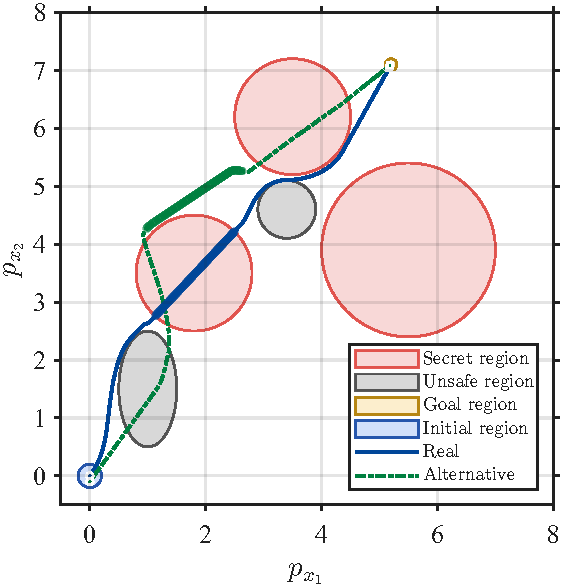
\includegraphics[scale=0.5]{fig/opacity10traj.pdf}
    \caption{Real and alternative trajectories under opacity.}
    \label{fig:opacity_traj}
\end{figure}
\begin{figure}[t]
    \centering
    \subfigure[Indistinguishability CBF]{
        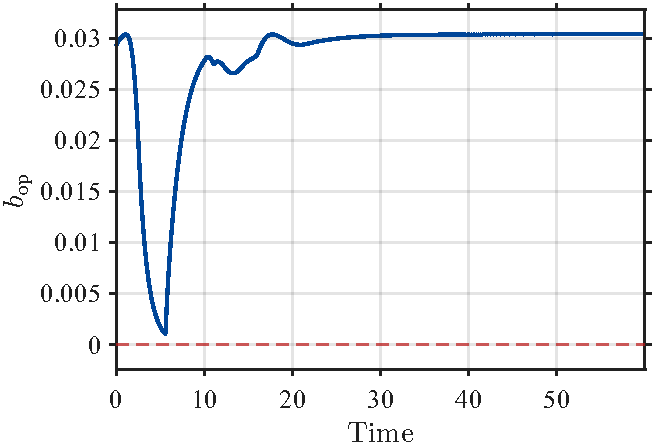
\includegraphics[width=0.227\textwidth]{fig/opacity10delta.pdf}
        \label{fig:traj}
    }
    \hfill
    \subfigure[Non-simultaneous secrecy CBF]{
        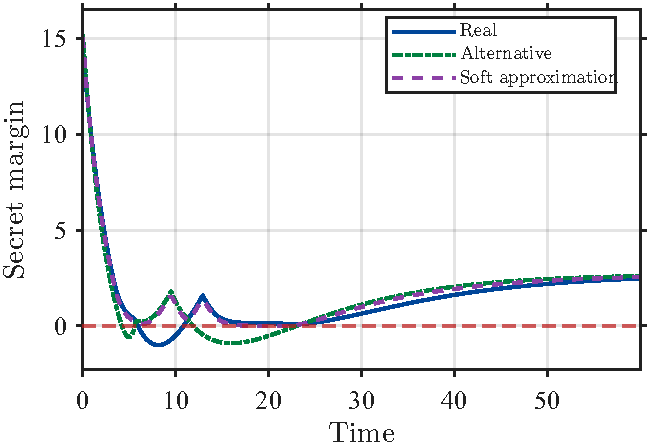
\includegraphics[width=0.227\textwidth]{fig/opacity10secret.pdf}
        \label{fig:ctrl}
    }
    \caption{CBF margins.}
    \label{fig:simulation}
\end{figure}

The real and alternative trajectories are initialized at $\mathbf{x}_{0, 1} = (0,0)$ and $\mathbf{x}_{0, 2} = (0, 0.1)$. The synthesized trajectories are shown in Fig.~\ref{fig:opacity_traj}. The real trajectory reaches the goal and avoids the unsafe regions, while the alternative one remains observationally close to the real one and non-secret whenever the real execution visits a secret region (thick lines in Fig.~\ref{fig:opacity_traj}). Hence, the intruder cannot infer secret visits from observations.

% \begin{figure}[tb]
%     \centering
%     \includegraphics[scale=0.5]{fig/ni0.4traj.pdf}
%     \caption{Real and alternative trajectories under noninterference.}
%     \label{fig:ni_traj}
% \end{figure}

% \begin{figure}[tb]
%     \centering
%     \includegraphics[scale=0.5]{fig/anonymity0.4traj.pdf}
%     \caption{Real and alternative trajectories under $K$-anonymity.}
%     \label{fig:anon_traj}
% \end{figure}

% \begin{figure}[tb]
%     \centering
%     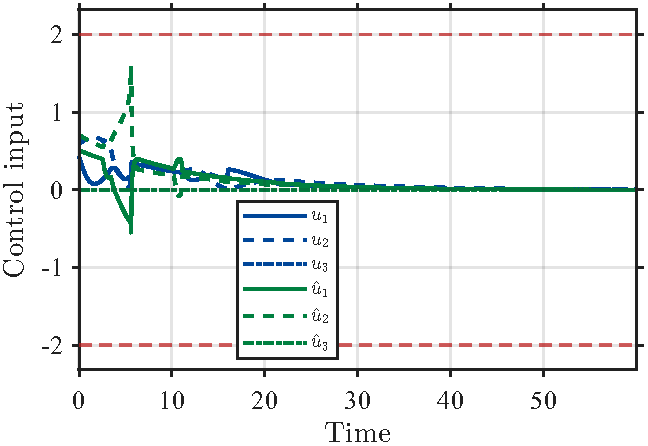
\includegraphics[scale=0.8]{fig/opacity10ctrl.pdf}
%     \caption{Control input}
%     \label{fig:ctrl}
% \end{figure}

% \begin{figure}[tb]
%     \centering
%     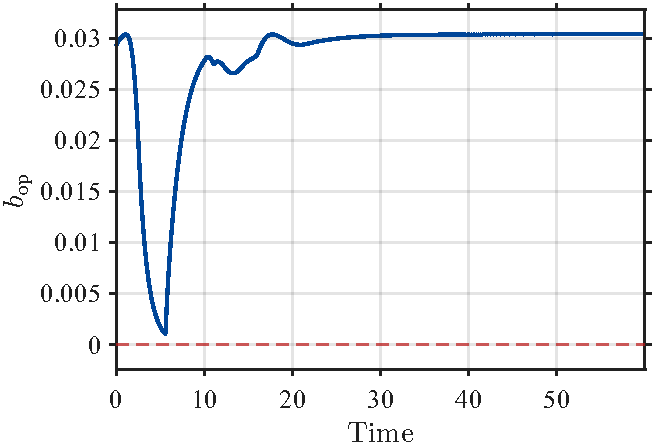
\includegraphics[scale=0.8]{fig/opacity10delta.pdf}
%     \caption{Indistinghuisability CBFs}
%     \label{fig:delta}
% \end{figure}

% \begin{figure}[tb]
%     \centering
%     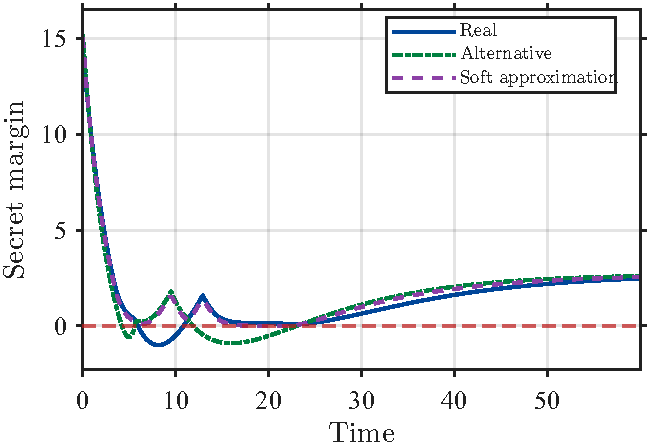
\includegraphics[scale=0.8]{fig/opacity10secret.pdf}
%     \caption{Secrecy CBFs}
%     \label{fig:secret}
% \end{figure}

% \begin{figure}[tb]
%     \centering
%     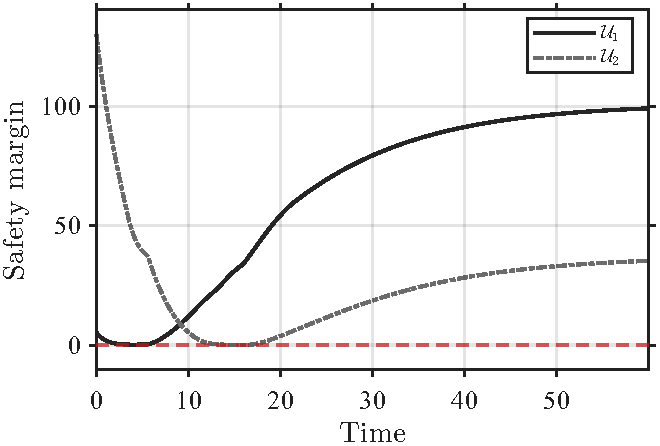
\includegraphics[scale=0.8]{fig/opacity10safety.pdf}
%     \caption{Safety CBFs}
%     \label{fig:safety}
% \end{figure}

\section{Conclusion}
\label{sec:conclusion}

This paper presents an online CBF-based framework for enforcing security hyperproperties in continuous-time CPS, with formal guarantees and demonstrated effectiveness in robot case studies. Future work includes extending the framework to more general classes of hyperproperties.
 
\bibliographystyle{IEEEtran}
\bibliography{Ref}


\end{document}